\section{Kryptografi}
\begin{frame}
\frametitle{Innehåll}
\tableofcontents[currentsection]
\end{frame}

\begin{frame}{Kryptografi}


\begin{columns}
    \begin{column}{0.45\textwidth}
        \begin{itemize}
			\item Historia
			\item Symmetrisk kryptering
			\begin{itemize}
				\item[-] Gemensam nyckel
			\end{itemize}
			\item Exempel
			\begin{itemize}
				\item[-] Caesar
				\item[-] Enigma
			\end{itemize}
		\end{itemize}
    \end{column}
	\begin{column}{0.55\textwidth}
    	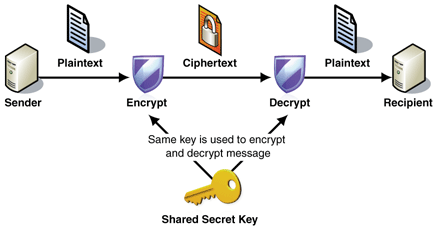
\includegraphics[width=\textwidth]{images/symmetric.png}
	\end{column}
\end{columns}

\end{frame}

\begin{frame}{Public Key Cryptography}

\begin{columns}
    \begin{column}{0.45\textwidth}
        \begin{itemize}
			\item Räddningen
			\item Diffie \& Hellman
			\item Olika nycklar
			\item Okända parter kan kommunicera
		\end{itemize}
    \end{column}
	\begin{column}{0.55\textwidth}
    	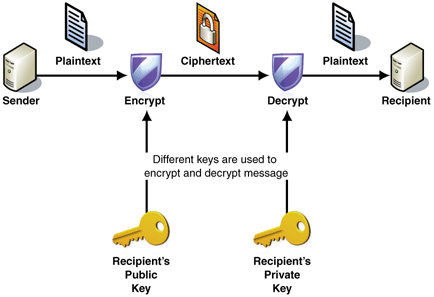
\includegraphics[width=\textwidth]{images/asymmetric.png}
	\end{column}
\end{columns}

\end{frame}

\begin{frame}{El Gamal-kryptografi}

\begin{columns}
	\begin{column}{0.5\textwidth}
		\begin{itemize}
			\item Givet y, g \& p, vad är x?
			\item Diskreta logaritmen svår
			\item Grunden i El Gamal-krypto
		\end{itemize}
	\end{column}
	\begin{column}{0.5\textwidth}
		{\LARGE $$y := g^x \mod{p}$$}
	\end{column}
\end{columns}

\vspace{3pt}

{\LARGE
\begin{align*}
y &\vcentcolon= g^{x} \,\,\,\,\,\,\,\,\,\, s\in \mathcal{R} \\
c &= (g^s, y^s\cdot m) = (u, v) \\
 m &= u^{-x}\cdot v
\end{align*}}

\end{frame}

\begin{frame}{Egenskaper hos El Gamal}

\begin{columns}
	\begin{column}{0.6\textwidth}
		\begin{itemize}
			\item Homomorft
			\begin{itemize}
				\item[-] Möjliggör flera lager kryptering
			\end{itemize}
			\item Generalisering till andra grupper
		\end{itemize}
	\end{column}
	\begin{column}{0.4\textwidth}
		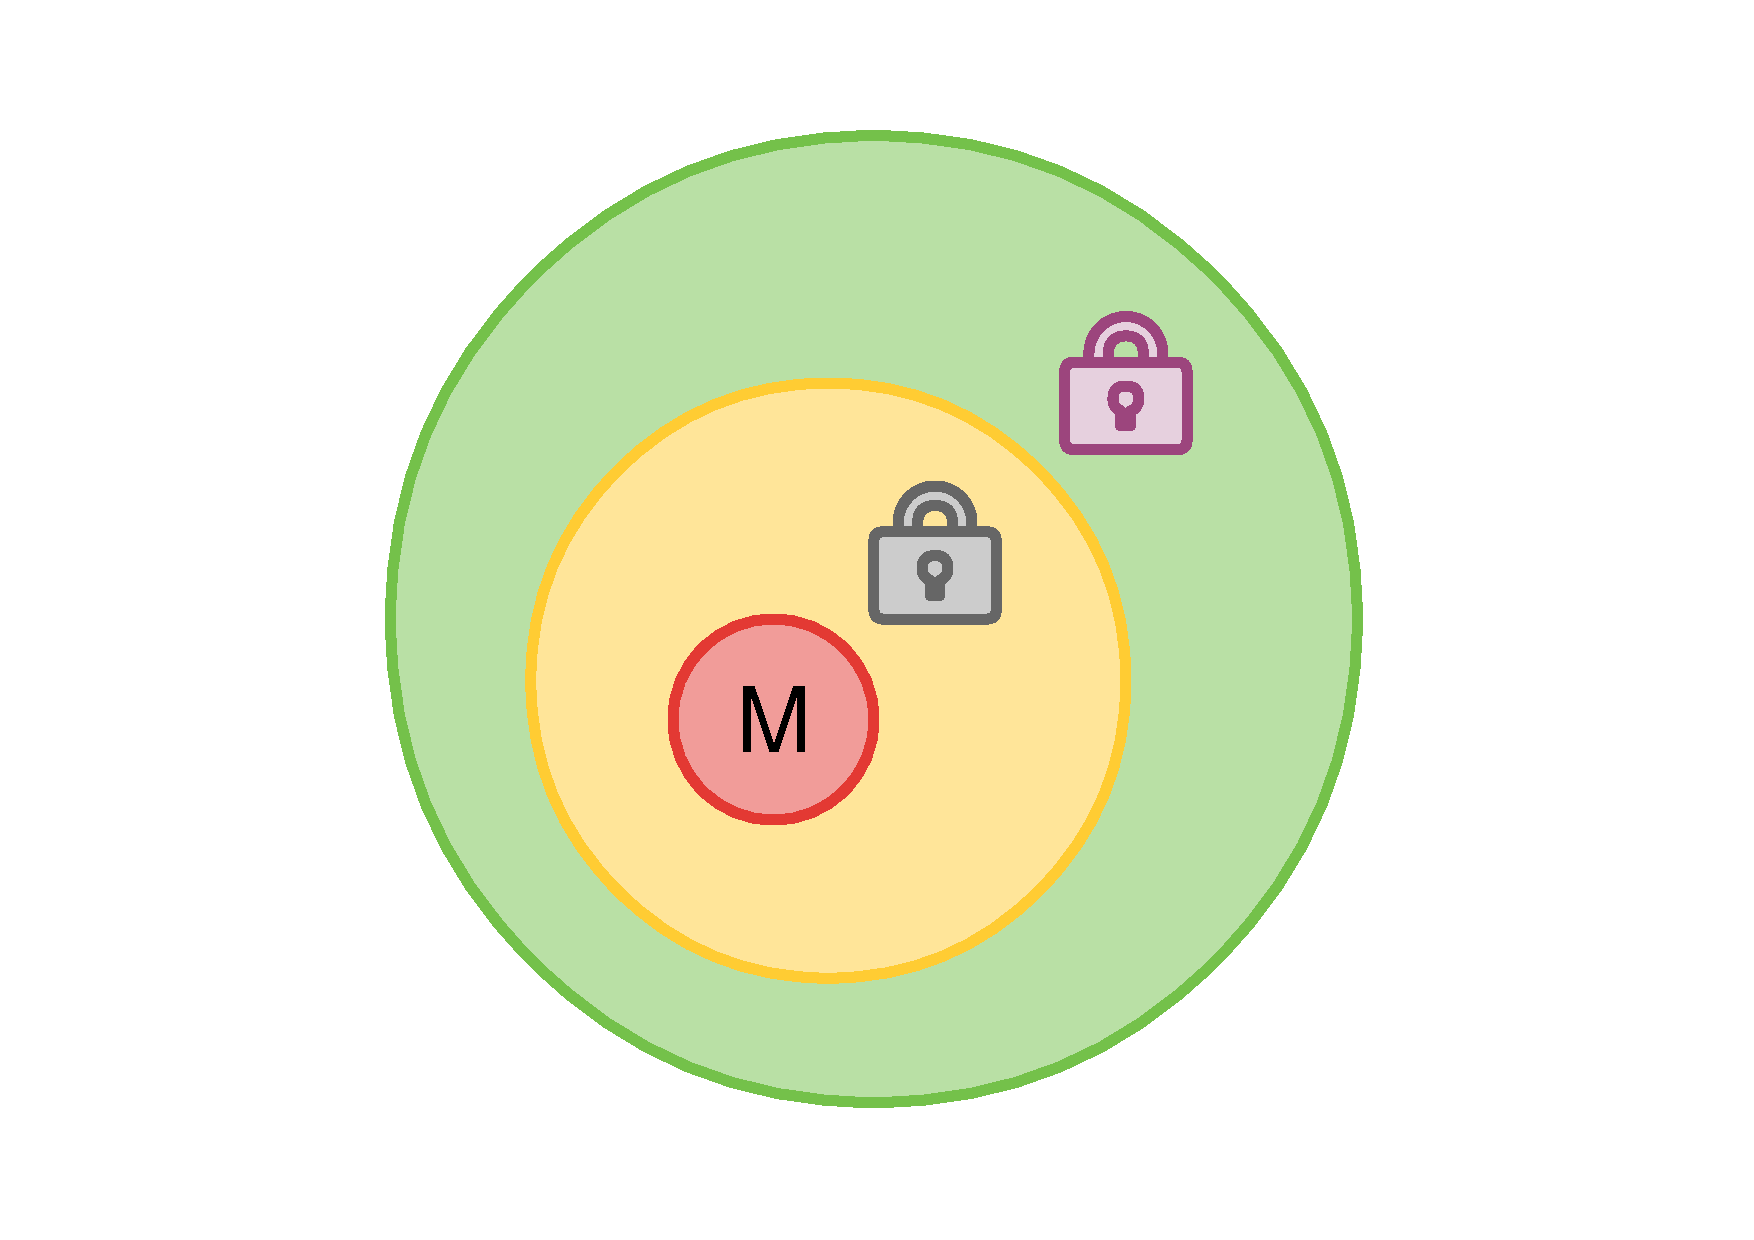
\includegraphics[width=\textwidth]{images/mix6.pdf}
	\end{column}
\end{columns}

\end{frame}

\begin{frame}{Zero-knowledge bevis}

\begin{itemize}
\item Bevis för ett påstende
\item Avslöjar inte något annat
\item Exempel
\begin{itemize}
	\item[-] Diskreta logaritmen
\end{itemize}
\end{itemize}

\end{frame}
